

	\section{Материалы}
	
	
	\begin{figure}[h]
	    \centering
	    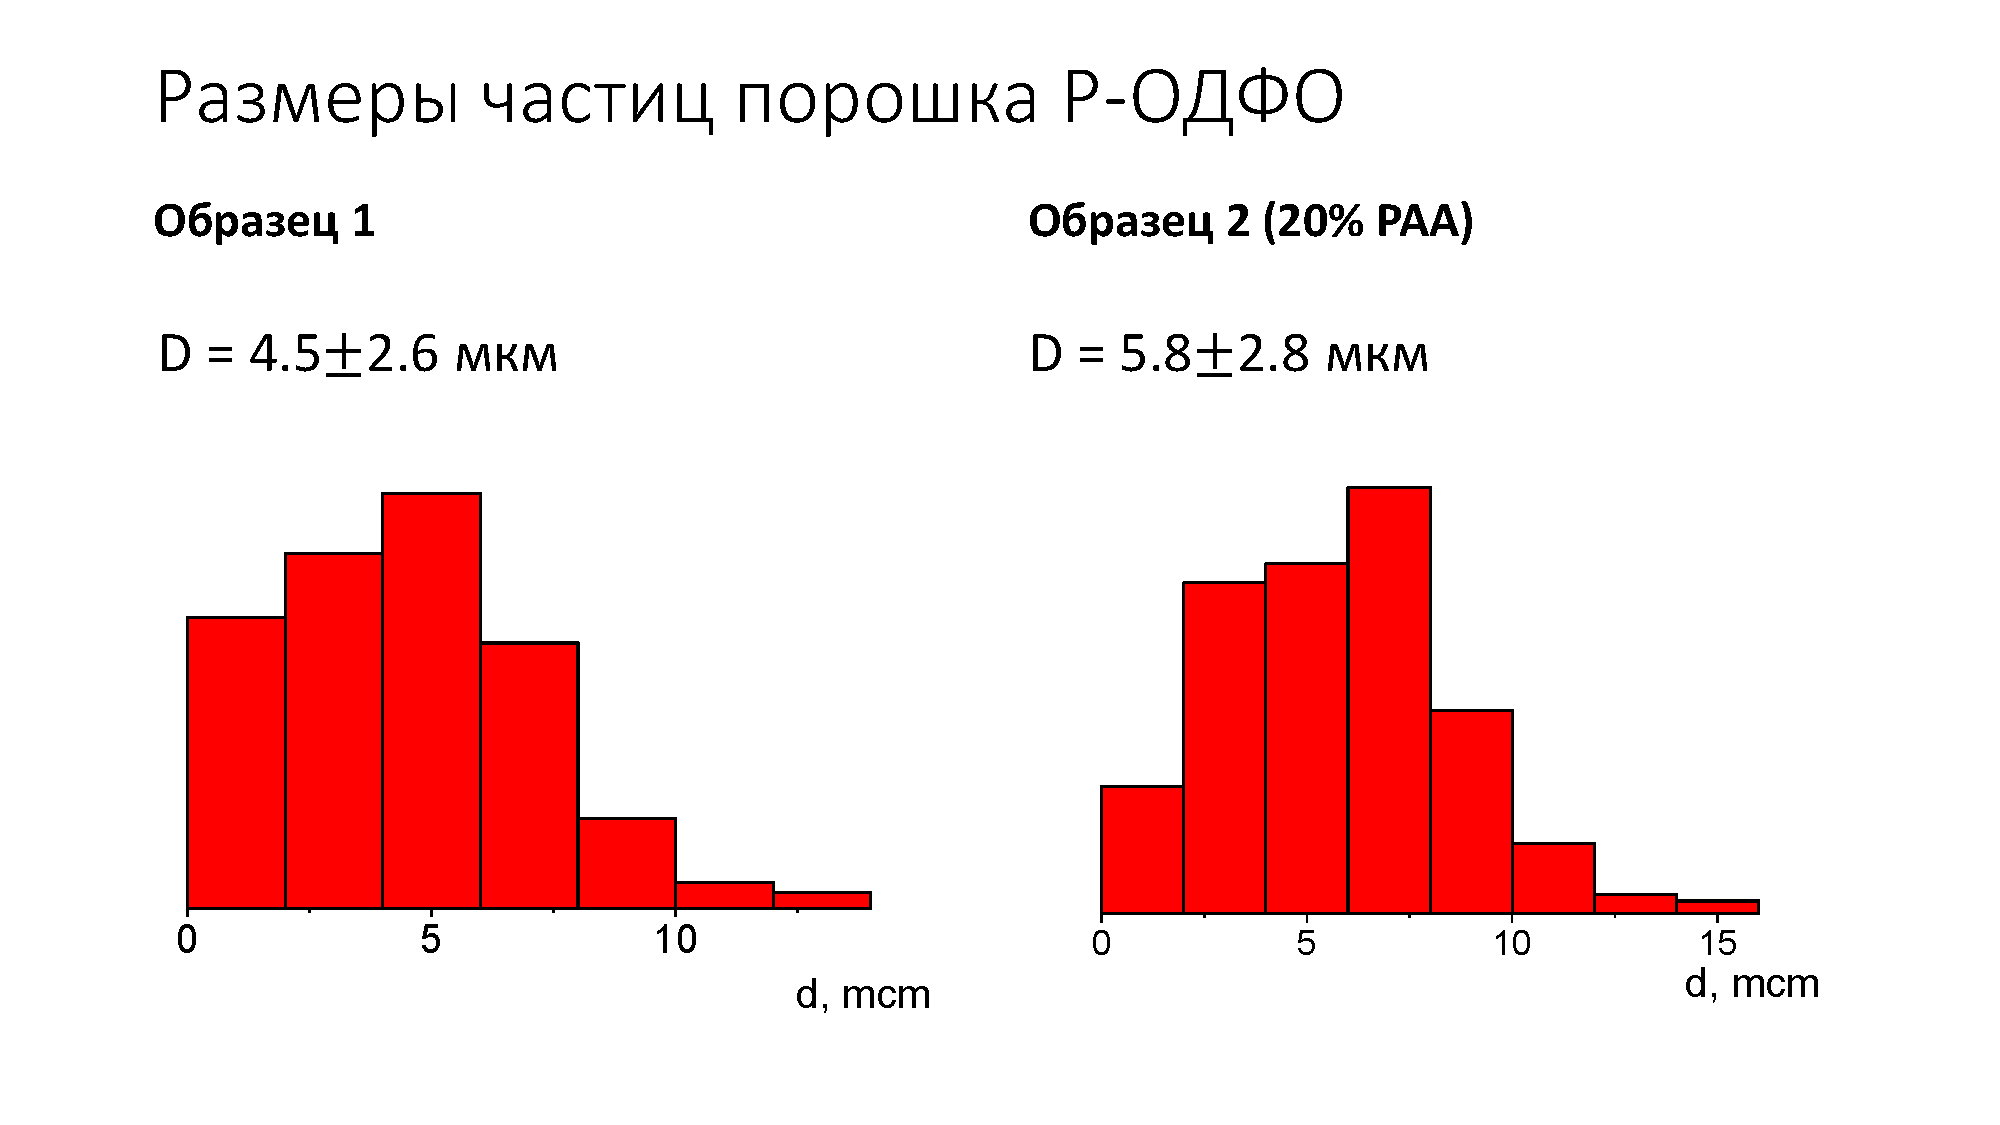
\includegraphics[width=\linewidth]{fig/particles}
	    \caption{Caption}
	    \label{fig:my_label}
	\end{figure}
	
	\section{Схема эксперимента}
	\subsection{Источник излучения}
	
	Измерения проводились на микрофокусной линии D13 Европейского центра синхротронного излучения (ERSF).
	
		\begin{figure}[h]\center
\begin{tabular}{cc}
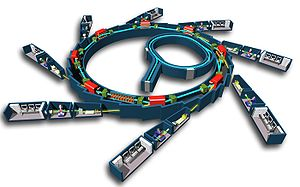
\includegraphics[width=0.5\linewidth]{fig/pribor-scheme.jpg}
&
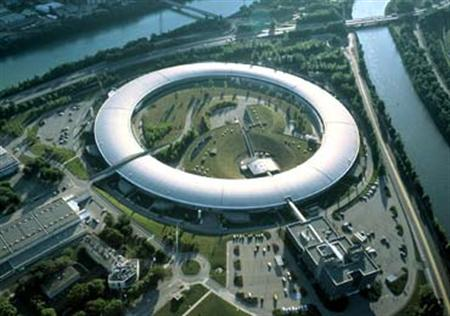
\includegraphics[width=0.5\linewidth]{fig/pribor-photo.jpg}
\end{tabular}
\caption{Синхротрон ERSF}
\end{figure}
	
\subsection{Микрофокусный сканирующий эксперимент}

	
	\section{Получение и первичная обработка данных}
	\paragraph{1D или 2D}
	
	\section{Вычитание фона, аппроксимация пиков}
	Распознавание кристаллических пиков и аморфного фона производилось с помощью алгоритма "Rolling ball". \\
	Принуип действи понятен из рис. \ref{fig:ball}
	
	\begin{figure}[h]
	    \centering
	    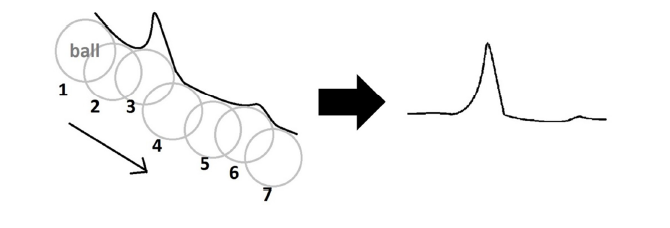
\includegraphics[width=\linewidth]{fig/ball.PNG}
	    \caption{Caption}
	    \label{fig:ball}
	\end{figure}
	Данный алгоритм применяется при анализе данных рентгеновской дифракции, рамановской спектроскопии и пр. []. Как правило он применяется к двумерным дифрактограммам кристаллических материалов, как например, в работе \cite{ball2018}. Однако подходящая реализация для одномерных профилей, необходимая в случае дифракции на полимерах, не представлена в открытых источниках. Ниже (листинг \ref{lst:ball}) приведена адаптация алгоритма из работы \cite{ball-code}, реализованная на языке Python. 
	
	
	\begin{lstlisting}[language=Python, caption=Python example, label={lst:ball}]
	
import numpy as np
 
def incmatrix(genl1,genl2):
    m = len(genl1)
    n = len(genl2)
    M = None #to become the incidence matrix
    VT = np.zeros((n*m,1), int)  #dummy variable
 
    #compute the bitwise xor matrix
    M1 = bitxormatrix(genl1)
    M2 = np.triu(bitxormatrix(genl2),1) 
 
    for i in range(m-1):
        for j in range(i+1, m):
            [r,c] = np.where(M2 == M1[i,j])
            for k in range(len(r)):
                VT[(i)*n + r[k]] = 1;
                VT[(i)*n + c[k]] = 1;
                VT[(j)*n + r[k]] = 1;
                VT[(j)*n + c[k]] = 1;
 
                if M is None:
                    M = np.copy(VT)
                else:
                    M = np.concatenate((M, VT), 1)
 
                VT = np.zeros((n*m,1), int)
 
    return M
\end{lstlisting}
	
	\section{Карты кристалличности}
	
	\section{Параметры решетки, расчеты}
	
	
	\paragraph{Rolling-ball}
	погрешности, чем хорошо, почему он, какие еще бывают
	


    \paragraph{фиттинг}

\begin{figure}
    \centering
    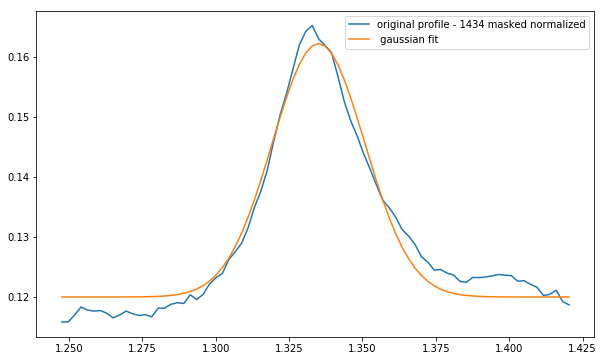
\includegraphics[width=\linewidth]{fig/gauss-fit.png}
    \caption{Аппроксимация формы пика по разным моделям}
    \label{fig:my_label}
\end{figure}
	
	\paragraph{Карты кристалличности}
	
	\begin{figure}[ht]\center
\begin{tabular}{cc}
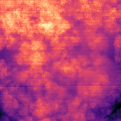
\includegraphics[width=0.5\linewidth]{fig/map-1.png}
&
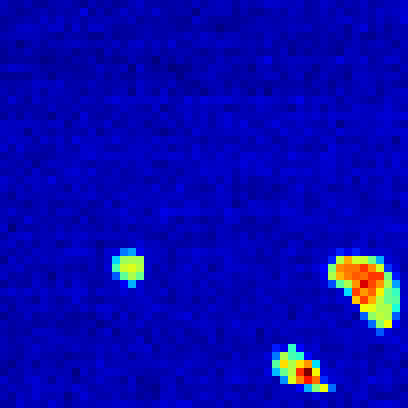
\includegraphics[width=0.5\linewidth]{fig/map-2.png} \\
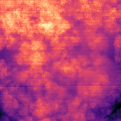
\includegraphics[width=0.5\linewidth]{fig/map-1.png}
&
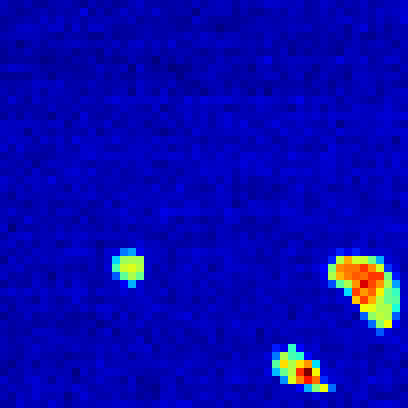
\includegraphics[width=0.5\linewidth]{fig/map-2.png}
\end{tabular}
\caption{Карты кристалличности}
\end{figure}
	
	

	
	
	
	Свойства и результаты прочих исследований:
	[Vaganov corrected]